\chapter{Ziele der Kryptologie}
Die Ziele der Kryptologie sind klar definiert, man spricht von drei bis vier Hauptzielen um Daten, Nachrichten und Übertragungskanäle geheim zu halten. Das erste Ziel der Kryptologie, sind die „Vertraulichkeit und Zugriffsrechte“, es bedeutet das nur autorisierte Personen Zugriff auf die Daten beziehungsweise in Computernetz versendete Nachrichten haben sollen, um private Daten oder Nachrichten lesen zu können. Anders formuliert, die Geheimhaltung einer Nachricht sollte erhalten werden. Das zweite Ziel ist die Integrität, also der Änderungsschutz, hierbei müssen alle Daten nachweislich vollständig und unverändert beim Empfänger ankommen. Das dritte Ziel ist die „Authentizität, Fälschungsschutz“, wichtig ist hier das der Urheber, also der Sender, eindeutig auf seine Nachricht identifizierbar ist, eine Fälschung der eigenen Identität also ausgeschlossen werden kann. Das bedeutet der Empfänger muss überprüfen können ob die Nachricht wirklich von dem Urheber stammt. Dieses Ziel ist schwer zum dritten Ziel zu unterschieden. In vielen Fachbüchern wird deshalb Authentizität und Verbindlichkeit unter einem Ziel zusammengefasst. Auch ich werde die Verbindlichkeit nicht explizit weiter behandeln und es auch zusammenfassend in das dritte Ziel integrieren, Grund hierfür ist unter anderem der „Platzmangel“ der Seminarfacharbeit. Das bedeutet hier wird das vierte Ziel nur Vollständigkeitshalber angesprochen, aber im weiterem Verlauf nicht weiter erläutert. So wird sich ausschließlich auf die ersten drei Ziele konzentriert. Um diese Ziele der Kryptologie erreichen zu können, und somit die Datensicherheit gewährleisten zu können, gibt es verschiedenste Methoden die wir im Vortext bereits erwähnt haben und auch in der Praxis Anwendung finden. Die Umsetzung wird fast ausschließlich durch mathematische Methoden, wie z.B. der Prüfsummen und technischen Funktionen umgesetzt. Die Ziele werden im Kapitel „Zusammenfassung“ auf unser Programm angewendet und näher erläutert. Bevor ich aber die Ziele der Kryptologie auf das RSA Verfahren anwenden kann, benötigen wir vorerst einen erweiterten Kenntnisstand über das RSA Verfahren. Ebenso benötigen wir das Wissen, wie mit Hilfe von Zielen der Kryptologie auch Datensicherheit gewährleistet werden kann. 

\section{Datenschutz und Datensicherheit}
Datenschutz ist eng mit der Kryptologie verbunden, weil sie ähnliche Ziele verfolgen. Anders formuliert, die Kryptologie wird verwendet um Datensicherheit gewährleisten zu können. Der allgemeine Grundsatz der Datensicherheit lautet, „Datensicherheit ist der Schutz von Daten vor Verfälschung, Zerstörung oder Verlust.“, Datenschutz hingegen beschäftigt mit dem Schutz des Persönlichkeitsrechts bei der Datenverarbeitung. Grundsätzlich sagt er aus, dass jeder selbst für seine Daten verantwortlich ist und selber entscheiden kann wen er welche Daten anvertraut. Der Datenschutz bezieht sich also eher auf die rechtlichen Aspekte, die im Kapitel „Kryptographie in Recht und Gesellschaft“ näher erläutert werden. Die Datensicherheit ist also grundlegender und für den technischen Aspekt wichtiger.\\

Hierbei kann die Datensicherheit durch Virenprogramme, Firewall, Passwortabfrage, aber natürlich auch mit den allgemeinen Verschlüsselungen erhalten werden. Verwendet werden diese Maßnahmen für Datenschutz und Datensicherheit um vor Viren, Würmer oder Trojanern schützen zu können. Die Vorbeugung solcher Angriffe bietet unter anderem auch die Kryptographie. Damit beispielsweise ein Fremdzugriff durch Trojaner auf die privaten Daten erschwert wird und ein sicherer Austausch von Daten gewährleistet werden kann. Es gibt somit verschiedenste Möglichkeiten seine Daten verschlüsseln zu können, um Fremdzugriff verhindern zu können. Die Verschlüsselung wird dennoch in unserer Seminarfacharbeit ausschließlich mit asymmetrischen Verschlüsselungen veranschaulicht und angewandt. Anzumerken ist aber, dass es natürlich noch andere Möglichkeiten gibt, z.B. durch die symmetrischen Verschlüsselungen Datensicherheit zu erreichen. \cite{Sicherheit}\\

\section{Ziel 1 und 2 der Kryptologie}
Um die Ziele der Kryptologie in Bezug auf die RSA Verschlüsselung beschreiben zu können, benötigt es ausführliches Wissen über den RSA Algorithmus. Alle Grundlagen des RSA Verfahrens wurden bereits im vorherigen Kapitel „Asymmetrische Verschlüsselung“ ausführlich erläutert. Der folgende Inhalt bezieht sich auf die Grundlagen der asymmetrischen Verschlüsselung.\\

Nun kann mit Hilfe des RSA Algorithmus Schlussfolgerungen für die Datensicherheit gezogen werden. Es gilt also zu klären, ob der RSA Algorithmus die Ziele der Kryptologie erfüllt. Um nun die Tauglichkeit der RSA zu überprüfen, wenden wir die bereits genannten 3 Ziele der Kryptologie an, finden tut man diese im Kapitel „Ziele der Kryptologie“. Nun mehr zur theoretischen Überprüfung der Ziele. Das erste Ziel wird klar erfüllt, denn nur berechtigte Personen haben die Möglichkeit auf eine RSA Verschlüsselung zuzugreifen, indem sie entweder „d“ wissen, oder einfach ausgedrückt „p1“ und „p2“ wissen. Der private Schlüssel ist also nur einsichtig für berechtigte Personen. Das bedeutet die Geheimhaltung wäre gewährleistet, da nur der Empfänger die verschlüsselte Nachricht einsehen kann. Ebenso ist zu empfehlen „p“ und „q“ nach der Schlüsselerzeugung zu vernichten, da nur mit ihnen eine Rekonstruktion des Schlüsselpaares möglich ist. Das zweite Ziel wird auch erfüllt, weil hier die eigentliche Zahl „d“ nicht verändert werden kann, außer man kennt als Dritter „p1“ und „p2“, dann wäre eine Veränderung von „d“ möglich und das Endergebnis wäre veränderbar. Aber um „d“ verändern zu können, benötigt der Angreifer entweder „n“, oder „p1“ und „p2“ und das ist sehr schwer herauszufinden, vorausgesetzt „n“ oder „p1“, „p2“ sind nicht leicht zu faktorisieren. Das bedeutet die Nachricht kann nur vor der Verschlüsselung mit dem öffentlichen Schlüssel noch verändert werden. Eine Veränderung der Nachricht nach der Verschlüsselung ist also nicht mehr möglich, nicht einmal für denjenigen, der die Nachricht verschlüsselt hat. \\

Denn nur der Empfänger besitzt den passenden privaten Schlüssel für seinen öffentlichen Schlüssel, dass bedeutet nur er ist in der Lage die Nachricht wieder zu entschlüsseln. Dennoch um beweisen zu können, dass die Nachricht verändert wurde, wird das Ziel abseits vom eigentlichen RSA Verschlüsselungsverfahren durch Anwendung von Hashes erzielt. Im nächsten Kapitel möchte ich speziell auf die Hashfunktion eingehen, weil diese auch von mir praktisch im Form eines Programmes angewendet wird.


\subsection{Hashes}

Hashes oder auch Hashfunktionen sind essentiell wichtig für die Kryptographie. Im Rahmen unserer Seminarfacharbeit wird sich auf den Anwendungsbereich der Integrität beschränkt. Im Prinzip ist die Hashfunktion eine kryptografische Prüfsumme für eine Nachricht, um Integrität gewährleisten zu können. Zur Verdeutlichung, in der Praxis wird eine beliebige Zeichenfolge erzeugt und durch die Hashfunktion in einen Hashwert beziehungsweise Prüfsumme „umgewandelt“ und verschickt. Nun erhält der Empfänger die Nachricht mit der Zeichenfolge und auch den dazugehörigen Hashwert. Aber der Empfänger möchte sicher gehen das der Text nicht verändert wurde, so vergleicht er die beiden Hashes, also vom Sender und Empfänger. Stimmen sie überein, dann ist keine Veränderung der Nachricht erfolgt und ist somit das Original. Ist der Hashwert anders, ist beim übertragen entweder die Nachricht manipuliert worden, oder es ist zu einer fehlerhaften Übertragung gekommen. Das alles wird ermöglicht durch einen Hashwert, der möglichst von jeden einzelnen „Nachrichtenbit“ abhängt. Das bedeutet, dass durch die kleinste Veränderung in der Zeichenfolge beziehungsweise des Textes eine große Änderung im Hashwert sich widerspiegeln sollte. Kommen wir nun zu einigen weiteren Eigenschaften die eine Hashfunktion besitzen sollte. Eine Hashfunktion basiert auf sogenannten Einwegfunktionen. Das heißt sie werden nur für einen bestimmten Zeitraum zur Verfügung gestellt. Grund hierfür ist unter anderem die mögliche Kollision zwischen Hashwerten. So kann es beispielsweise vorkommen, dass es zufälligerweise zwei identische Hashwerte gibt, um das aber verhindern zu können, werden heutige Hashalgorithmen mit einer Länge mit bis zu 160 Bit ausgestattet und zeitlich begrenzt, z.B. MD5- Message Digest 5. Ebenso darf die Umkehrung einer Hashfunktion, also die Ermittlung der Nachricht zu einem gegebenen Hashwert nicht möglich sein. Wichtig ist auch zu erwähnen das der Hashwert in der Praxis separat verschlüsselt wird, da sonst eine Änderung der Hashes im Text der verändert wurde, die Gefahr besteht, dass der Hashwert angeglichen werden könnte und so eine Verfälschung der Nachricht sich nicht im eigentlichen Hashwert widerspiegeln würde. Hashes bieten also viele Vorteile die auch in der RSA Verschlüsselung ihre Anwendung finden. Nun habe ich mich dafür entschieden eine Hashfunktion auf das RSA Verfahren anzuwenden. Um mögliche beweise und Entschlüsse für RSA im allgemeinen und unseren Programmen zu verdeutlichen. \\

\subsection{Hashfunktion und deren Anwendung}
Nachdem ich mich intensiv mit der RSA Verschlüsslung und dessen mathematischen Kontexten beschäftigt habe, bin ich nun in der Lage ein Programm mit Hilfe der Programmiersprache Java zu schreiben. Voraussetzung für das volle Verständnis wird im Kapitel „Asymmetrische Verschlüsselung“ erlangt, indem sich intensiv mit den mathematischen Kontexten des RSA Verfahrens auseinandergesetzt wird. Hierbei stand im Mittelpunkt herauszufinden, ob und wie man eine Hashfunktion in einem Programm umsetzten kann, um das Ziel der Integrität gewährleisten zu können. Um damit Rückschlüsse auf die allgemeine Tauglichkeit von RSA schließen zu können. Zweitens wird in diesem Abschnitt nur das Programm erläutert. Ergebnisse werden im Kapitel „Tauglichkeitsuntersuchung“ präsentiert. Der Quelltext ist im Anhang zu finden, im nachfolgenden Text werden Zeilenangaben des Quellcodes angegeben, um alles nachvollziehen zu können. Das Programm wird in 3 Klassen untergliedert. Die Klassen Vars.java, SetFuncs.java, Hash.java. Die Klasse Vars.java legt alle Variablen fest, diese für die Implementierung des RSA Algorithmus benötigt werden. Diese lauten „p,q,N,e,c,d,M“. Die Bezeichnung der Variablen werden fast in jeder Literatur die sich mit RSA beschäftigt verwendet und auch im Anhang erläutert, unter Glossar. Hierbei werden alle Variablen auf private und „int=0“ gesetzt, außer M mit den Datentyp char. Char deswegen, weil als Veranschaulichung nur ein Zeichen verschlüsselt wird, also ein char und kein String. Ebenso werden hierfür für alle Variablen „set und get Methoden“ festgelegt. Die „set und get Methoden „werden benötigt um die einzelnen Variablen einlesen und „verwenden“ zu können. In der Klasse SetFuncs.java, hier werden alle Methoden zur Berechnung für den RSA Algorithmus implementiert. Es werden auch nicht alle Funktionen im folgenden Text ausführlich erläutert, da ich sonst den Rahmen der Seminarfacharbeit nicht einhalten könnte. Da aber jede Funktion essentiell wichtig ist, wird jede Funktion im Anhang im Quelltext nochmals kurz kommentiert. Nicht nur die Funktionen spielen einzeln wichtige Rollen. So ist es wichtig sie auch untereinander und einzeln zu überprüfen, ob sie die Bedingungen für die einzelnen Variablen erfüllen. Werden die Bedingungen nicht erfüllt, wird das Programm abgebrochen, weil der RSA Algorithmus sonst nicht „funktionell“ funktionieren würde. Das bedeutet die Funktionen gewährleisten, dass die Richtlinien mathematischer Kontexte eingehalten werden. In Zeile 26 des Quellcodes wird die Befehlssammlung für die Hashfunktion MD5 erzeugt, die für die Erzeugung des Hash benötigt wird. In Zeile 32 wird die Befehlssammlung in ein Bytearray eingelesen. In Zeile 35-39 werden Teile des Substrings mit Hilfe des Stringbuilders an diesen angehangen. In Zeile 62-70 wird die Funktion zur Berechnung des „ggT“, größter gemeinsamer Teiler, ermittelt, also „e“.Zeile 80-82 prüft mit „boolean“ ob die Bedingung des „ggT“ erfüllt werden. In Zeile 90-97 wird mit einer „for Schleife“ in der Gleichung 1=(e*d) mod ((p-1)*(q-1)) geprüft, ob ein Wert von 0-20 als „d“ in Frage kommen würde. In Zeile 110-112 wird ein „char“, also ein Zeichen beziehungsweise „M“ für die Verschlüsselung eingegeben. In Zeile 120-137 wird geprüft ob es sich hierbei um eine Primzahl oder nicht handelt, also ob es sich hierbei um eine natürliche Zahl handelt, die größer als eins und ausschließlich durch sich selbst und durch eins teilbar ist. In Zeile 144-189 finden noch weitere Überprüfungen statt, die für eine Anwendung des RSA Algorithmus benötigt werden. Das bedeutet es wird geprüft ob „e“ teilerfremd zu „p“ und „q“ ist, ebenso wird geprüft ob „p“ und „q“ nicht die gleichen Primzahlen sind. Es wird also der Zusammenhang der Variablen und Funktionen untereinander überprüft. Nun zur dritten Klasse Hash.java, die nun die Funktionen, Variablen benutzt und anwendet. In Zeile 17 wird ein Objekt erstellt was die Funktionen lädt, dass bedeutet hier findet keine Vererbung im eigentlichen Sinne statt. In Zeile 20-32 werden „p,q,e“ eingegeben. In Zeile 35 wird der private Schlüssel erzeugt, also d. In Zeile 38 wird der öffentliche Schlüssel, also „N“ erzeugt. In Zeile 41 wird eine Nachricht eingegeben, also ein Zeichen durch char, also „M“. In Zeile 47 wird nun mit den eben genannten Funktionen die Nachricht verschlüsselt. Ebenso wird „M“ vorher noch umgewandelt, vorerst in einen String und dieser dann in ein int Wert. Da „$A^24$“ nicht lösbar ist. So werden die einzelnen Zeichen mit Hilfe der ASCII Tabelle in int Werte umgewandelt. In Zeile 52 - 54 erfolgen die Ausgaben mit dem jeweiligen Hash und der verschlüsselten und entschlüsselten Nachricht. Diesen Hashwert könnte man sich vormerken und mit der veränderten Nachricht vergleichen. Um die Hashwerte vergleichen zu können, um Rückschlüsse auf eine mögliche Manipulation schließen zu können.

\subsection{Ziel 3 der Kryptologie}
Das dritte Ziel kann auch erzielt werden. Nun kann die RSA Verschlüsslung aber grundsätzlich keine Authentizität gewährleisten. Um das Problem lösen zu können, hilft sich die Kryptographie mit den sogenannten digitalen Signaturen aus. Das bedeutet jede Nachricht ist auf einen Benutzer zu 100\% zuzuordnen. Das wird ermöglicht, durch den sogenannten virtuellen Fingerabdruck. Er gibt jeder Nachricht eine individuelle Erkennbarkeit. Dabei ist wichtig das keine sichere Datenübertragung nur mit digitalen Signaturen erreicht werden kann, es ist nämlich trotzdem eine Verschlüsslung notwendig. So kommen wir zu Problemen der Authentizität bei den RSA Verfahren. Es ist nämlich nicht direkt möglich bei einer RSA Verschlüsslung herauszufinden, ob es sich beim Sender wirklich um die Person handelt, oder ob er seine Identität fälscht. Das bedeutet das Ziel der Authentizität kann vorerst nicht erreicht werden. Nun ist es aber möglich RSA im Grundprinzip auf ein Signaturverfahren „umzumünzen“. Das bedeutet es wird ermöglicht die Schlüssel zu vertauschen. Dennoch werden wir im Rahmen unserer Seminarfacharbeit nicht spezieller auf den Algorithmus des Signaturverfahrens mit RSA eingehen. Um eine digitale Signatur mit dem Prinzip der RSA erreichen zu können wird wie bereits erwähnt die Funktion der Schlüssel getauscht. So wird hierbei mit dem privaten Schlüssel verschlüsselt und mit dem öffentlichen Schlüssel entschlüsselt. Und weil der private Schlüssel bekanntlich nur einer Person zugeordnet werden kann, ist die Nachricht nachweislich zu 100\% von der Person der mit diesem privaten Schlüssel eine Nachricht verfasst hat. Dadurch wäre die Authentizität gewährleistet. Die Nachricht wird dann mit dem öffentlichen Schlüssel entschlüsselt. Nun ist hierbei die Authentizität und Integrität gewährleistet, aber nicht mehr die eigentliche Geheimhaltung. So ist es nun jeden möglich die verschlüsselte Nachricht mit dem öffentlichen Schlüssel zu entschlüsseln und zu lesen. Man kann also festhalten das das RSA Verfahren mehrere Anwendungsmöglichkeiten bietet. Zum einen kann man „geheim“ verschlüsseln und zum anderen eine digitale Signatur erstellen. Dennoch besteht auch eine sehr komplexe Möglichkeit, die ermöglicht beides gleichzeitig anzuwenden. Wir haben uns aber bewusst gegen ein Programm entschieden, welches digitale Signaturen und gleichzeitig die Geheimhaltung gewährleisten soll, weil wir sonst den fachlichen Rahmen zu weit ausgebreitet hätten und somit auch jeglichen Rahmen einer Seminarfacharbeit. Somit beschränken wir uns auf die Geheimhaltung. Es gibt auch mehrere Sicherheitsprobleme bei den digitalen Signaturen der RSA, diese auf mathematische Kontexte zurückzuführen sind, dennoch ich im Rahmen unserer Seminarfacharbeit nicht weiter ausführen möchte. Die eben genannten „komplexen“ Möglichkeiten finden ihren Anklang vor allem in der Praxis, da sie die eben genannten Vorteile mitbringen.

\section{RSA in der Praxis}
In der Praxis findet das RSA Verfahren Anklang bei den digitalen Signaturen, wie PGP, Pretty Good Privacy“ und SSH, „Secure Shell“. Hierbei werden sie oft in Form von Hybriden Verschlüsselungen angewendet, also Verschlüsselungen die zum Beispiel symmetrische und asymmetrische Verfahren kombinieren. Die RSA Verschlüsselung benötigt für große Datenmengen aber viel zu viel Zeit. Das hat zur Folge, dass die RSA Verschlüsslung nicht direkt bei Verschlüsselungen für große Datenmengen zur Anwendung kommt, sondern eher zum verschlüsseln des „kleinen“ Saison-Keys der symmetrischen Verschlüsselung. Um es kurz zu fassen, es werden Nachrichten mit großen Datenmengen, mit Hilfe des symmetrischen Verschlüsselungsverfahren verschlüsselt und weil das noch keine ausreichende Sicherheit gewährleisten würde, wird der Schlüssel der symmetrischen Verschlüsselung mit einem asymmetrischen Schlüssel zusätzlich verschlüsselt. Somit wird das langsame asymmetrische Verfahren, welches für große Daten äußerst lange braucht, nicht eingesetzt. Dafür verschlüsselt man mit dem asymmetrischen Verfahren, den Schlüssel des symmetrischen Verfahrens, da die Schlüssel nur aus kleinen Datenmengen bestehen. Abschließend ist zu sagen, dass asymmetrische Verschlüsselungen gänzlich ungeeignet sind für reine Geheimhaltungen von großen Datenmengen, sie werden meistens in Kombination mit anderen Methoden eingesetzt, weil sonst die eben genannten Nachteile überwiegen. Es gibt noch zahlreiche andere Funktion, die ich aber im Rahmen unserer Seminarfacharbeit nicht weiter aufgreifen werde.

\section{Kryptoanalyse}
Bevor ich mich mit der Kryptoanalyse beschäftige muss gesagt werden, dass ich nicht alle Angriffsmethoden nennen und erläutere. Denn nur alleine die Kryptoanalyse würde genügend Informationen für noch eine Seminarfacharbeit bieten. So gebe ich einen grundlegenden Überblick über die Kryptoanalyse und gehe auf ein Verfahren näher ein.\\

Soeben wurden Möglichkeiten aufgezeigt, wie man sich mit Hilfe von Verschlüsselungsmethoden, mit beispielsweise RSA schützen kann und somit unbefugten Personen Eintritt auf private Nachrichten verweigert werden können. Nun aber zum zweiten großen Teil der Kryptologie, die Kryptoanalyse. Diese beschäftigt sich nicht mit der Entwicklung neuer Methoden, sondern wendet schon bereits vorhandene Methoden an, um diese auf Schwachstellen abzusuchen und mögliche Sicherheitslücken finden zu können. Mit dem Ziel die verwendete Verschlüsselungsmethode zu stärken und von Sicherheitslücken befreien zu können. Anders formuliert: „Analyse und Bewertung der Sicherheit von Kryptoverfahren gegen unbefugte Angriffe“.\\

Besonders für meinen Eigenanteil ist die Kryptoanalyse sehr wichtig, weil ich in der Rolle eines Kryptoanalytiker handle und das RSA Verfahren in Bezug auf unsere Programme auf Tauglichkeit untersuche. So ist eine Tauglichkeitsuntersuchung durch einen Kryptoanalytiker besonders wichtig in der heutigen Zeit, um Schwachstellen eines Programmes vor der Veröffentlichung ausfindig zu machen. Nun kann natürlich Kryptoanalyse nicht nur zur Stärkung von Programmen genutzt werden, sondern meist wird Kryptoanalyse von „Angreifern“ genutzt, die das Ziel verfolgen ein verschlüsseltes Programm beziehungsweise Nachricht zu entschlüsseln, indem er zum Beispiel den geheimen Schlüssel herausfindet. Aber auch andere Sicherheitslücken können genutzt werden, so kann es beispielsweise vorkommen, dass der Angreifer nicht einmal einen Schlüssel benötigt um an die geheimen Informationen zu kommen. Das wäre das sogenannte „Worse-Case“ eines Programmes und zeichnet ein nicht ausreichend getestetes Programm aus. Es gibt verschiedene Möglichkeiten um an den geheimen Schlüssel zu gelangen.\\

\subsection{Angriffsverfahren durch Kryptoanalyse}
Nun zu einigen „gängigen Methoden“. Zum Beispiel der known Ciphertext, Known Plaintext, Chosen Plaintext und Chosen Ciphertext Angriff. Aufgrund des „Platzmangels“ können die eben genannten Verfahren nicht weiter erläutert werden. Dennoch wird sich mit einer Methode näher beschäftigt und zwar mit dem Bruce-Force Angriffsverfahren. In der Bruce-Force Angriffsmethode wird versucht den Schlüssel durch schlichtes probieren zu ermitteln. Natürlich nicht mit Stift und Papier, sondern mit Computern. Heutzutage wird hierfür viel Rechenleistung benötigt, um Möglichkeiten des Schlüssels „durchzuspielen“. Ein Beispiel wäre, nimmt man einen Schlüssel mit der Schlüssellänge von 25 Bit, hätte man $2^25$ Möglichkeiten, also 33.554.432 Möglichkeiten. Nun nehmen wir an, wir bräuchten 2 Sekunden um eine Kombination eines Schlüsselpaares auszuprobieren. Man bräuchte also maximal ca. 776 Tage, also ca. 2 Jahre bis man alle Möglichkeiten ausprobiert hätte und somit auch zu 100\% den Schlüssel hätte. Wichtig hierbei anzumerken ist, dass auch gleich beim ersten Versuch der Schlüssel gefunden werden könnte, oder auch erst beim letzten. Des Weiteren werden in der Praxis abseits von den theoretischen Methoden natürlich vor allem trojanische Pferde benutzt um an bestimmte geheime Schlüssel zu gelangen, aber auch kann man jemanden gezielt ein geschwächtes Verschlüsselungsverfahren „anvertrauen“, um daraus seinen Erfolg zu erzielen. Zum Beispiel ein Programm entwickeln, welches mit Sicherheitslücken an eine Organisation weiterverkauft wird. Die Kryptoanalyse bietet somit viele Möglichkeiten um Verschlüsselungen zu umgehen. Alles was man im Prinzip braucht, ist Geduld, ein „Verfahren“, Rechenleistung und natürlich auch ein wenig Glück. Hierbei möchte ich den Begriff Rechenleistung und deren Bedeutung noch einmal näher erläutern. In den letzten Jahren sind die Computer immer schneller geworden.\\
Nun erschwert folgendes Szenario die Verschlüsselungsmethode der RSA, mit der wir uns auch im Eigenanteil intensiv beschäftigen. Wie wir bereits geklärt haben, besteht diese Verschlüsselungsmethode im Prinzip auf der Geheimhaltung zweier Primzahlen. Nun könnte man aus der Sicht eines Kryptoanalytikers durch „probieren“ die Primzahlen ermitteln. Das geht natürlich umso schneller, desto schneller auch der Computer rechnen kann. Das bedeutet, wenn die Rechenleistung von Rechnern stetig steigt, müssen natürlich auch die Primzahlen größer werden.

\subsection{Brute-Force Angriffsmethode und deren Gefahren}
Im Kapitel „Angriffsverfahren durch Kryptoanalyse“ wurde geklärt was ein Bruce-Force Angriff ist und welche Gefahren entstehen können. Nun möchte ich zur Verdeutlichung meines zweiten Programmes, welches das Bruce-Force Verfahren veranschaulicht, den mathematischen Hintergrund kurz beleuchten. In dieser Erläuterung geht es um das Problem von zu klein gewählten Primzahlen in einer RSA Verschlüsselung. Grundsätzlich ist eine Veränderung der Verschlüsselung der RSA-Methode nur möglich, wenn der Wert „d“ bekannt ist, somit gibt es natürlich Möglichkeiten diesen herauszufinden. Man kann durch bestimmte Software, z.B. mein Programm, den privaten Schlüssel ermitteln. Denn sind „p1“ und „p2“ ermittelt worden, kann man „n“ errechnen und mit Hilfe von „n“ kann man „d“ errechnen. Wichtig anzumerken ist noch, dass unser Programm grundsätzlich auf kleinen Primzahlen beruht, also selbst durch vorhandene Software „relativ“ schnell eine Lösung gefunden werden kann. Das bedeutet um zu verhindern, dass man das Produkt von „n“ herausfindet, nimmt man Zahlen die nicht leicht zu faktorisieren sind. Um ein Beispiel zu nennen, $p1=2^30$, $p2=2^35$, nun soll man aus diesen beiden Faktoren das unbekannte Produkt „n“ finden, weil ja n=(p1-1) *(p2-1), hier wird es den Angreifer um einiges schwieriger gemacht das Produkt „n“ zu finden um später „d“ ermitteln zu können. Aus diesem Grund ergibt sich ein Richtwert für Schlüssellängen. So ist für einen asymmetrischen Schlüssel mindestens eine Länge von 1024-2048 Bit oder 3072 Bit zu wählen. Für die längerfristige Sicherheit sollten die Schlüssel eine Länge von 15360 Bit haben. Man kann also festhalten, dass der Bruce-Force Angriff durch die massive Rechenleistung, bei Verschlüsselungssystemen mit kurzen Schlüsseln eine echte Bedrohung darstellt. Ausschließlich mit langen Schlüsseln kann man sich gegen die Bruce-Force Angriffe schützen. Der Bruce-Force Angriff eignet sich also ideal um eine Schwachstelle der RSA zu veranschaulichen. Deswegen habe ich mich dazu entschieden die Bruce-Force Angriffsmethode und deren Gefahren für das Verschlüsselungsverfahren der RSA, mit Hilfe eines „Demo Programms“ zu beweisen.

\subsection{Bruce-Force Programm}
Die Simulation des Bruce-Force Programms erfolgt ebenso in einem Java Programm, was ganz normal von Netbeans ausgeführt werden kann. Die Erstellung des RSA Algorithmus ist identisch zum Hash Programm und wird somit in das Programm übernommen. Das „Demo Programm“ arbeitet mit einer festgelegten „size“, die auf genau 4 Bit festgelegt ist. Nun werden Eingaben von „p“, „q“ und „e“ abgefragt, die von einem Benutzer eingegeben werden sollen um schlussendlich damit ein Zeichen „m“ zu verschlüsseln. Im Programm wird versucht „p“ und „q“ zu errechnen um „n“ errechnen zu können. Wenn „p“ und „q“ ermittelt worden sind, kann nun damit ohne Probleme „d“ errechnen werden. Im Programm wird die Ermittlung mit zwei „verschachtelten „for Schleifen““ umgesetzt. Das bedeutet der jeweilige „x“, „y“ Wert wird nacheinander erhöht, bis die passenden Primzahlen, die eingegeben Primzahlen gefunden worden sind.

\section{Tauglichkeitsuntersuchung}
Erarbeitung des Eigenanteils aus Sicht eines Kryptoanalytikers. Dabei gehe ich wie folgt vor. Ich werde das erarbeitete theoretische Wissen, durch die Literatur, praktischen Anwendungen und durch selbst entwickelte Programme zusammenfassen und eine „Tauglichkeitstabelle“ ausarbeiten. Ziel der Tabelle ist es, den Nutzer erstens schnell einen Überblick über die wichtigsten Merkmale der Verschlüsselung zu vergegenwärtigen und zweitens Programme auf die Tabelle anwenden zu können, umso eventuell Schwachstellen für seinen eigenen Algorithmus finden zu können. Also unseren eigens programmierten Algorithmus auf Tauglichkeit zu testen. Die Tauglichkeitsuntersuchung wird in verschiedene Bereiche untergliedert, auf die die Tauglichkeitstabelle wie eine Checkliste angewendet wird. Nach der Untersuchung der Tauglichkeit der einzelnen Bereiche, wird eine Gesamtwertung der Programme erfasst und ausgewertet. Die Tabelle wird nicht alle Themengebiete die erarbeitet worden sind abdecken, da wir sonst den Rahmen der Seminarfacharbeit „sprengen“ würden. Es ist zu erwähnen das alles, was in der Tabelle verwendet wird, nicht auf alle Verschlüsselungen sinnvoll und logisch ist. Die Tabelle bezieht sich also grundsätzlich auf die asymmetrische Verschlüsslung, wie das RSA Verfahren. Ebenso ist alles sehr theoretisch und in der Praxis nicht immer umsetzbar und logisch. Dennoch werden mit zwei Programmen auch praktische Anwendungen veranschaulicht. Um aber in der Lage zu sein, eine Tauglichkeitsuntersuchung des Verfahrens der RSA von einem selbst erstellten Programm durchführen zu können, benötigen wir das Wissen aus den bereits erarbeiteten Kapiteln, speziell die Ziele der Kryptologie, Schwachstellen durch Kryptoanalyse und ausführliches Wissen über das Verfahren der RSA. \\
Zu Anfang kann ich festhalten, dass eine Verschlüsslung in der Lage sein sollte, so viele Ziele der Kryptologie wie möglich gewährleisten zu können. Um die Datensicherheit garantieren zu können. Ebenso sollte eine Verschlüsslung einen brauchbaren Schutz vor Angreifern und Schutz vor den gängigsten Angriffsmethoden haben. So werden folgende Bereiche bei der Tauglichkeitsuntersuchung mit einfließen. Die drei Ziele der Kryptologie, die Kryptoanalyse durch das Bruce-Force Angriffsverfahren veranschaulicht, ebenso werden praktische Aspekte mit aufgeführt. Aber vorher ist noch wichtig anzumerken, dass es sich zwar primär um unser Hauptprogramm handelt, dass das RSA Verfahren anwendet, dennoch ich Teilprogramme bilden musste. Ich habe mich also entschieden sogenannte „Demo-Programme“ zu erstellen. Der Grund ist die Komplexität des Hauptprogramms, die wir überschreiten würden, wenn wir keine Auslagerungen des Hauptprogramms durch „Demo Programme“ vorgenommen hätten. Das bedeutet wir hätten den Rahmen unserer Seminarfacharbeit mehrfach überschritten. Ebenso ermöglichen mir die „Demo Programme“ einzelne bestimmte Aspekte verdeutlichen und beweisen zu können, in Bezug auf die „Tauglichkeitsuntersuchungen“ des RSA Verfahrens. Weitere inhaltliche Gründe für die Auslagerung vom Hauptprogramm finden sie im fortlaufenden Text. Beginnen wir nun mit den Zielen der Kryptologie. Ich kann die Ziele der Kryptologie mit Hilfe der Programme und theoretischen Wissen über das RSA Verfahren beweisen und widerlegen. So habe ich unseren Algorithmus, der auf der Grundlage der RSA Verschlüsslung arbeitet, intensiv getestet. So bin ich diesbezüglich zum Entschluss gekommen, dass unsere Programme manche Ziele erfüllen und andere wiederum nicht. Hierbei gibt es keinerlei Abweichung zum theoretisch erarbeiteten Wissen, welches bereits im Kapitel „Ziele der Kryptologie“ erarbeitet und ausführlich erläutert wurde. Dort wurde erläutert wieso und weshalb manche Ziele erreicht und andere nicht erreicht werden können, dieser Erkenntnisgewinn spiegelt sich voll und ganz in unseren Programmen wieder und kann somit von mir bewiesen werden. So habe ich festgestellt, dass das erste Ziel der Kryptologie, was besagt das alle Daten nur von autorisierten Personen gelesen werden können, erfüllt wird. Das erste Ziel wird erfüllt, weil unser Programm auf der Grundlage der RSA Verschlüsselung arbeitet und so in der Lage ist einen Text sicher zu verschlüsseln, also der Text ohne privaten Schlüssel nicht zu entschlüsseln ist, somit ist die Geheimhaltung gewährleistet. Des Weiteren habe ich festgestellt, dass auch das zweite Ziel der Kryptologie, was besagt das alle Daten beim Empfänger unverändert seien müssen, erfüllt ist. Hierbei ist aber wichtig anzumerken, dass das Ziel theoretisch bereits dadurch erfüllt wird, weil die RSA Verschlüsslung es mathematisch kaum ermöglich die Primzahlen herauszufinden, wenn sie denn groß genug sind. Dennoch kann ich zusätzliche Beweise liefern. Bewiesen wird es durch ein Hilfsprogramm, was sogenannte Hashes von MD5 verwendet, dass ausführlich erläutert worden ist. So wird es ermöglicht jede Nachricht mit einem Hashwert auszustatten. Das bedeutet jede Nachricht ist abhängig von jedem einzelnen Bit der Nachricht. \\
Durch mehrere Tests des Programmes wurde festgestellt, dass die kleinste Veränderung einer Nachricht eine große Änderung des Hashwertes widerspiegelt und eine Manipulation der Nachricht somit bewiesen werden kann. Voraussetzung hierfür war, den Hashwert der Nachricht vom Sender zu notieren und ihn nach der Ausführung der Verschlüsselung mit diesen zu vergleichen. Da jedes Zeichen einen anderen Hashwert hat, beweist, dass eine veränderte Nachricht auch einen anderen Hashwert haben würde. Das heißt wir konnten nicht während der Verschlüsselung den Hashwert überprüfen, dass bedeutet ein realistischer Manipulationsangriff wurde nicht simuliert, dennoch würde jemand einen Angriff ausführen, würde sich nun aber die Nachricht ändern, demnach auch ein völlig anderer Hashwert entstehen. Ebenso wird bei jeder Nachricht ein neuer Hashwert generiert und eingesetzt. Es werden also die grundlegenden Richtlinien der Hashfunktionen erfüllt, diese bereits im Kapitel „Hashes“ erläutert worden sind, dennoch haben wir eine zeitliche Begrenzung der einzelnen Hashwerte nicht eingebaut. Die Funktion würde keinerlei Sinn ergeben in unseren „Demo Programm“, denn doppelte Hashwerte im Bereich von 160 Bit sind extrem unwahrscheinlich. Würde man das „Demo Programm“ jedoch im „World Wide Web“ anbieten, müsste natürlich aus Sicherheitsgründen eine zeitliche Begrenzung der einzelnen Hashwerte erstellt werden. So kann man festhalten, dass Hashfunktionen für die Integrität sehr wichtig sind. Denn sie sorgen dafür das Manipulationen unabhängig von der eigentlichen „Schutzfunktion“ der RSA Methode nochmals abgesichert werden und zeitgemäß geschützt werden können. Kommen wir nun zum dritten Ziel der Kryptologie, dass besagt das eine Nachricht eindeutig auf eine Person zurückzuführen ist. Das Ziel kann durch unser Programm nicht erreicht werden, aber auch nicht in der Theorie. Außer die Funktion wird durch den bereits erläuterten Schlüsseltausch oder Hybride Verschlüsselungen ermöglicht. Hierbei ist besonders wichtig zwischen zwei Varianten der RSA Verschlüsslung zu unterscheiden. Denn entweder man verschlüsselt seine Nachricht mit dem Verfahren, wie wir es erläutert und umgesetzt haben oder aber man benutzt den RSA Algorithmus, um eine digitale Signatur zu erstellen, um das dritte Ziel erfüllen zu können. Dabei hat alles seine Vorteile und Nachteile die bereits erläutert wurden. Da wir uns aber auf die allgemeine RSA Verschlüsslung konzentriert haben, kann das Ziel leider nicht erreicht werden. Nun kommen wir zu einem wichtigen Teil der Kryptologie und zwar zur Kryptoanalyse. Ich habe mich entschieden die Bruce-Force Angriffsmethode und deren Gefahren auf die RSA Verschlüsslung virtuell mit Hilfe eines weiteren „Demo Programms“ zu beweisen. Auch hier musste wieder eine Auslagerung vom eigentlichen Hauptprogramm vorgenommen werden. Grund ist, weil unserer Hauptprogramm ausschließlich nur mit abstrakten Klassen und Zahlen arbeitet, also nur zur Veranschaulichung des RSA Algorithmus. \\
Um aber mit Zahlen arbeiten zu können, um die Berechnung der Primzahlen zu ermöglichen, musste ich eine Auslagerung des Hauptprogramms vornehmen, die ich zur Veranschaulichung des Bruce-Force Angriffsverfahren essentiell benötige. Mit dem zweiten „Demo Programm“ ist es gelungen, dass Bruce-Force Angriffsverfahren simulieren zu können, dabei bin ich zu folgenden Entschlüssen gekommen. Die Bruce-Force Angriffsmethode ist zwar eine simple Methode, aber trotzdem eine der gefährlichsten Angriffsmethoden in Bezug auf RSA Verschlüsselungen mit kleineren Primzahlen, wie es im „Demo Programm“ der Fall ist. So stellt das Bruce-Force Verfahren eine große Gefahr dar und mit Hilfe des „Demo Programms“ kann bewiesen werden, dass das RSA Verfahren mit kleinen Schlüsseln leicht zu knacken ist. So können kleine Schlüssel, von 1 bis 4 Bit binnen weniger Stunden oder Tagen errechnet werden und so steht einer Manipulation der Nachricht nichts mehr im Wege. Anzumerken ist, dass es sich hier um einen Rechner mit eher mittelmäßiger Rechenleistung handelte, dass bedeutet die Berechnung von „p“ und „q“ würde mit anderen Rechnern durchaus schneller gehen. Die Tests konnten „innerhalb von Java“ nur bis 32 Bit getestet werden, weil Java nur bis zu 32 Bit, das entspricht der Dezimalzahl 2147483647, des Datentyps Integer unterstützt. Nochmals anzumerken ist, dass das Problem nicht mehr besteht, sobald größere Schlüssel verwendet werden. So wie bei unseren Hauptprogramm, welches eine Schlüssellänge von 1024 Bit beinhaltet. So ist statistisch gesehen unser Hauptprogramm zeitgemäß geschützt. Eine 2048 Bit Schlüssellänge, welches sicherer und zukunftssicherer wäre, haben wir nicht eingesetzt. Der Grund ist simpel, wir hätten durch die Berechnung eines solchen Schlüssels und mit der Verschlüsselung eines Textes ein vielfaches der Zeit benötigt. Abschließend kann festgehalten werden, dass das zweite „Demo Programm“, was die Bruce-Force Angriffsmethode simuliert, beweist, dass zu kleine Primzahlen zu einem erheblichen Sicherheitsrisiko, in der Verschlüsselung mit dem RSA Verfahren, beitragen würde. So kann abschließend festgehalten werden, dass die Programme sich verhältnismäßig gut schlagen. So werden die ersten beiden Ziele der Kryptologie erzielt und garantieren damit die Geheimhaltung der Texte, sowie die Integrität. Was zwar für Anwendungen in der Praxis eher schlecht ist, welches im Kapitel „RSA in der Praxis“ bereits beschrieben wurde, aber für unsere Seminarfacharbeit, die sich auf effektive Verschlüsselung und Geheimhaltung konzentriert völlig akzeptabel ist. So ist es möglich einen beliebigen Text einer Datei effektiv zu verschlüsseln, ebenso durch das „Hash Demo Programm“ wird noch die Absicherung durch die bereits genannten Hashes ermöglicht, welches ermöglicht die kleinste Änderung in einer Nachricht effektiv sichtbar zu machen. Dieses Programm arbeitet zwar unabhängig vom Hauptprogramm, könnte aber dennoch sofort in das Hauptprogramm integriert werden. Grund das es nicht integriert ist, ist die Komplexität des Hauptprogramms die einen Rahmen der Seminarfacharbeit „sprengen“ würde. \\
So erfüllt unser Hauptprogramm alleinstehend nicht „perfekt“ das zweite Ziel der Kryptologie, dennoch aber durch die Ergänzung des „Demo Programmes“ für Hashes, wird das Ziel unter „Vermerk“ komplett und souverän erfüllt. Es ist also gelungen den Algorithmus der RSA in Java-Code umzusetzen und so viele Ziele der Kryptologie, wie es ein Rahmen der Seminarfacharbeit erlaubt, zu erfüllen um Datensicherheit gewährleisten zu können. Ebenso beweise ich als aktiver Kryptoanalytiker, dass unser Programm einen Bruce-Force Angriff standhalten würde. Indem ein „Angriff“ mit dem Bruce-Force Verfahren simuliert wurde um zu beweisen, dass die Gefahr ausschließlich von kleinen Schlüssellängen ausgeht. Da unser Programm aber mit einer ausreichenden Schlüssellänge arbeitet, ist das Programm dahingehend sicher. Um zum Schluss zu kommen. Die Programme eignen sich nicht in der Praxis. Die Geheimhaltung und Integrität wird zwar erfüllt, was für eine Verschlüsselung ohne Authentizität ausreichend wäre, also für Nachrichten die keine große Priorität hätten. Dennoch würden sie einfach viel zu lange benötigen um einen Text, mit großer Datenmenge, erfolgreich zu verschlüsseln, auch wenn schon alles dafür getan wurde um Zeit bei der Verschlüsselung zu sparen. Indem die Schlüssellänge auf 1024 Bit begrenzt worden ist. Die einzige Aushilfe würden Hybride Verschlüsselungen bieten, mit denen man auch Authentizität gewährleisten könnte, diese aber aus Gründen der Komplexität nicht zur Anwendung kommen. Einen zusammenfassenden Überblick über die eben genannten Schlussfolgerungen der Tauglichkeit in Bezug auf die Programme finden sie im Abbildungsverzeichnis unter „Abbildung 3“ oder unter der Tauglichkeitstabelle. Ebenso ist wichtig zu erwähnen, dass ich die Seitenzahl leider nicht einhalten konnte, weil eine Tauglichkeitsuntersuchung mit wenigeren Aspekten, als ich aufgeführt habe, nicht aussagekräftig genug wäre. Ebenso ist zu erwähnen, dass bereits intensiv gekürzt worden ist. Eine weitere Kürzung würde also den inhaltlichen Rahmen zerstören und nicht aussagekräftig machen.

\begin{center}
	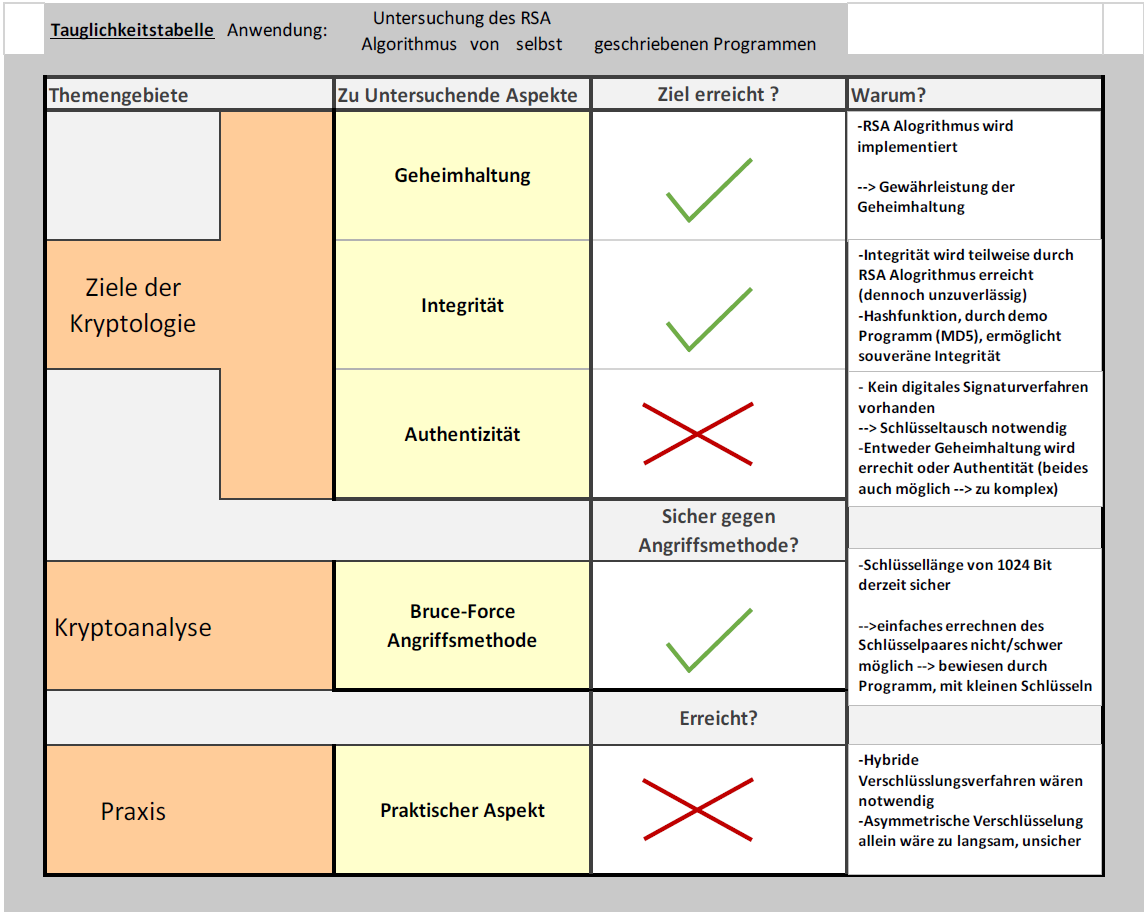
\includegraphics[width=1\textwidth]{./img/tauglichkeit}
	\captionof{figure}{\label{fig:tauglichkeit} Tauglichkeitsanalyse}
\end{center}